%%This is a very basic article template.
%%There is just one section and two subsections.
\documentclass{article}

\usepackage{a4wide}
\usepackage{amsmath}
\usepackage{float}
\usepackage{listings}
\usepackage{graphicx}
\usepackage{epstopdf}

\lstset{ %
breaklines=true,
language=R
}

\begin{document}

\title{Probability and Statistics for Data Analysis\\Assignment 2}
\author{Charalampos Kaidos}

\maketitle

\section{}
In the spreadsheet named Data 1 of the file Assignment 3 data.xlsx (available on
e-class assignments site) you will find the recorded variables $Y, X_1, X_2,
X_3$ (continuous) and $W$ (categorical with three levels) on 150 cases. Using
these data answer the following questions:

\subsection{}
Run the parametric one-way ANOVA of each of the continuous variables ($Y, X_1,
X_2, X_3$) on the categorical variable ($W$). Specifically,

\subsubsection{}
Provide a graphical representation of each of the continuous versus the
categorical variable

\begin{figure}[H]
\centering
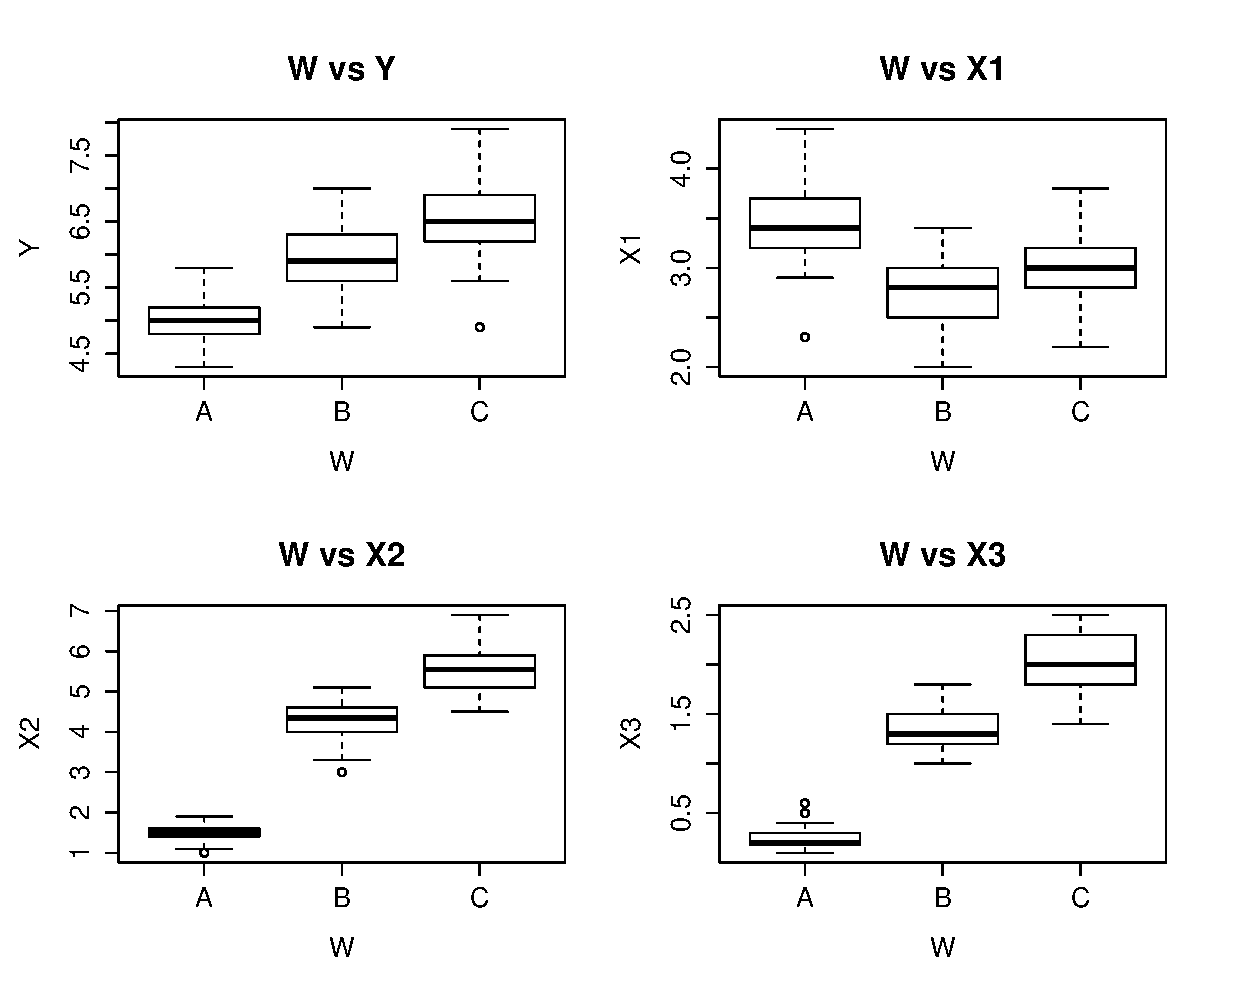
\includegraphics[scale=0.6]{valuesvsW.eps}
\caption{Continuous vs Categorical}
\label{fig:valuesvsW}
\end{figure}

\subsubsection{}
Provide the ANOVA output


\begin{enumerate}
  \item W vs Y
  \begin{lstlisting}
"Fitted model:"
Call:
   aov(formula = data[[col]] ~ factor(W), data = data)

Terms:
                factor(W) Residuals
Sum of Squares   63.21213  38.95620
Deg. of Freedom         2       147

Residual standard error: 0.5147894
Estimated effects may be unbalanced
  \end{lstlisting}
  
  \begin{lstlisting}
"Anova table:"
             Df Sum Sq Mean Sq F value Pr(>F)    
factor(W)     2  63.21  31.606   119.3 <2e-16 ***
Residuals   147  38.96   0.265                   
---
Signif. codes:  0 ‘***’ 0.001 ‘**’ 0.01 ‘*’ 0.05 ‘.’ 0.1 ‘ ’ 1
  \end{lstlisting}
  
  According to the ANOVA table above, the Y variable does not have the same mean
  for all values of W. This is also clear on the plot in figure~\ref{fig:YvsW}
  (p.~\pageref{fig:YvsW}).
  
  \begin{figure}[H]
  \centering
  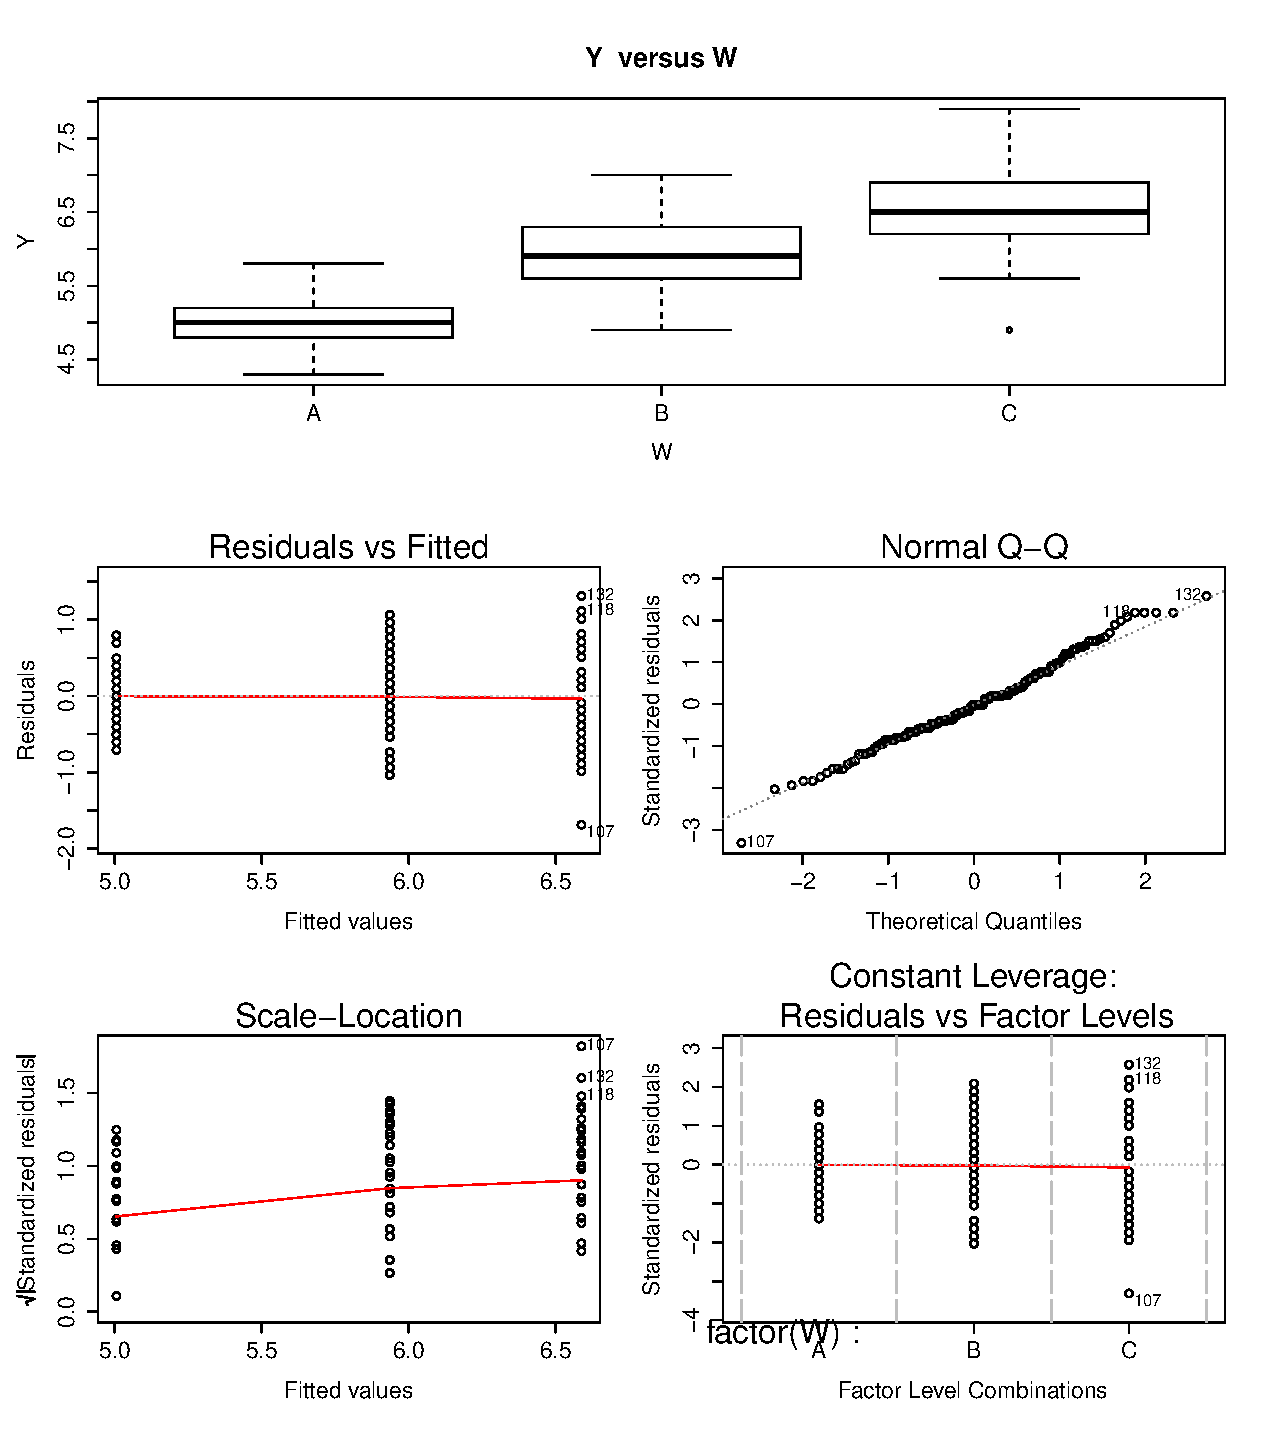
\includegraphics[scale=0.6]{YvsW.eps}
  \caption{W vs Y}
  \label{fig:YvsW}
  \end{figure}

  \item W vs X1
  \begin{lstlisting}
"Fitted model:"
Call:
   aov(formula = data[[col]] ~ factor(W), data = data)

Terms:
                factor(W) Residuals
Sum of Squares   11.34493  16.96200
Deg. of Freedom         2       147

Residual standard error: 0.3396877
Estimated effects may be unbalanced
  \end{lstlisting}
  
  \begin{lstlisting}
"Anova table:"
             Df Sum Sq Mean Sq F value Pr(>F)    
factor(W)     2  11.35   5.672   49.16 <2e-16 ***
Residuals   147  16.96   0.115                   
---
Signif. codes:  0 ‘***’ 0.001 ‘**’ 0.01 ‘*’ 0.05 ‘.’ 0.1 ‘ ’ 1
  \end{lstlisting}
  
  According to the ANOVA table above, the X1 variable does not have the same
  mean for all values of W. This is also clear on the plot in
  figure~\ref{fig:X1vsW} (p.~\pageref{fig:X1vsW}).
  
  \begin{figure}[H]
  \centering
  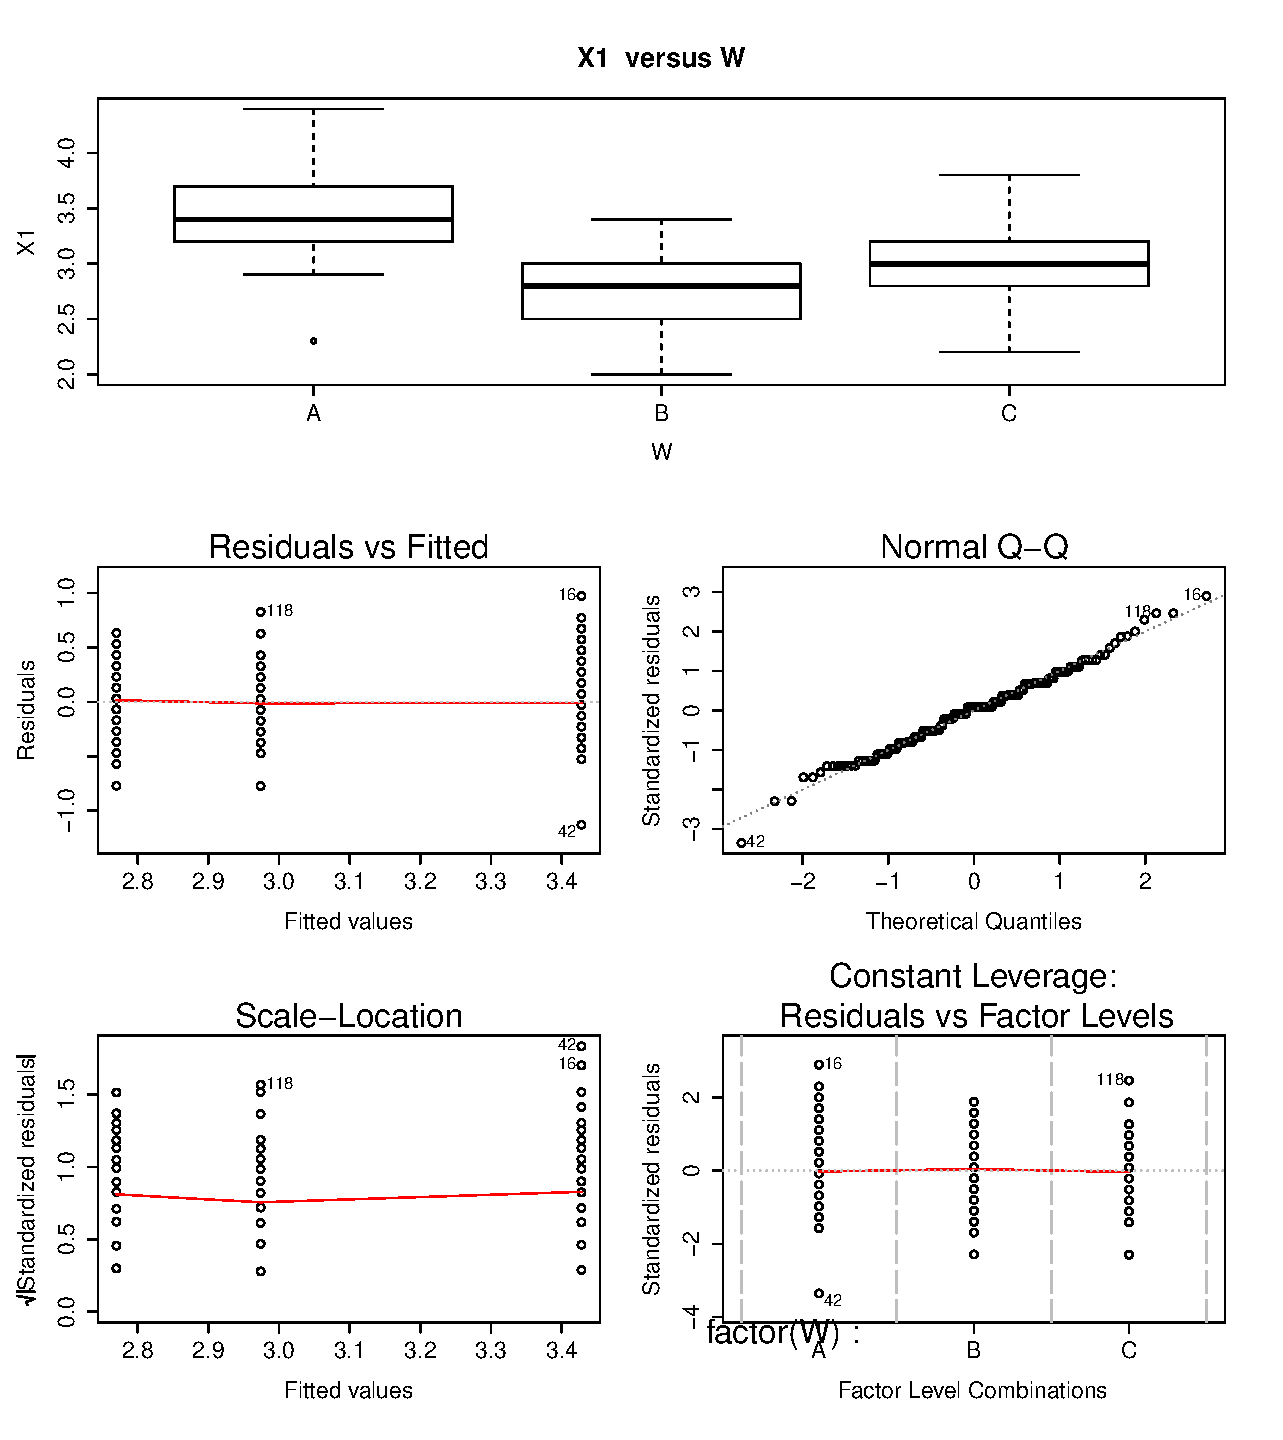
\includegraphics[scale=0.6]{X1vsW.eps}
  \caption{W vs X1}
  \label{fig:X1vsW}
  \end{figure}
  
  \item W vs X2
  \begin{lstlisting}
"Fitted model:"
Call:
   aov(formula = data[[col]] ~ factor(W), data = data)

Terms:
                factor(W) Residuals
Sum of Squares   437.1028   27.2226
Deg. of Freedom         2       147

Residual standard error: 0.4303345
Estimated effects may be unbalanced
  \end{lstlisting}

  \begin{lstlisting}
"Anova table:"
             Df Sum Sq Mean Sq F value Pr(>F)    
factor(W)     2  437.1  218.55    1180 <2e-16 ***
Residuals   147   27.2    0.19                   
---
Signif. codes:  0 ‘***’ 0.001 ‘**’ 0.01 ‘*’ 0.05 ‘.’ 0.1 ‘ ’ 1
  \end{lstlisting}
  
  According to the ANOVA table above, the X2 variable does not have the same
  mean for all values of W. This is also clear on the plot in
  figure~\ref{fig:X2vsW} (p.~\pageref{fig:X2vsW}).
  
  \begin{figure}[H]
  \centering
  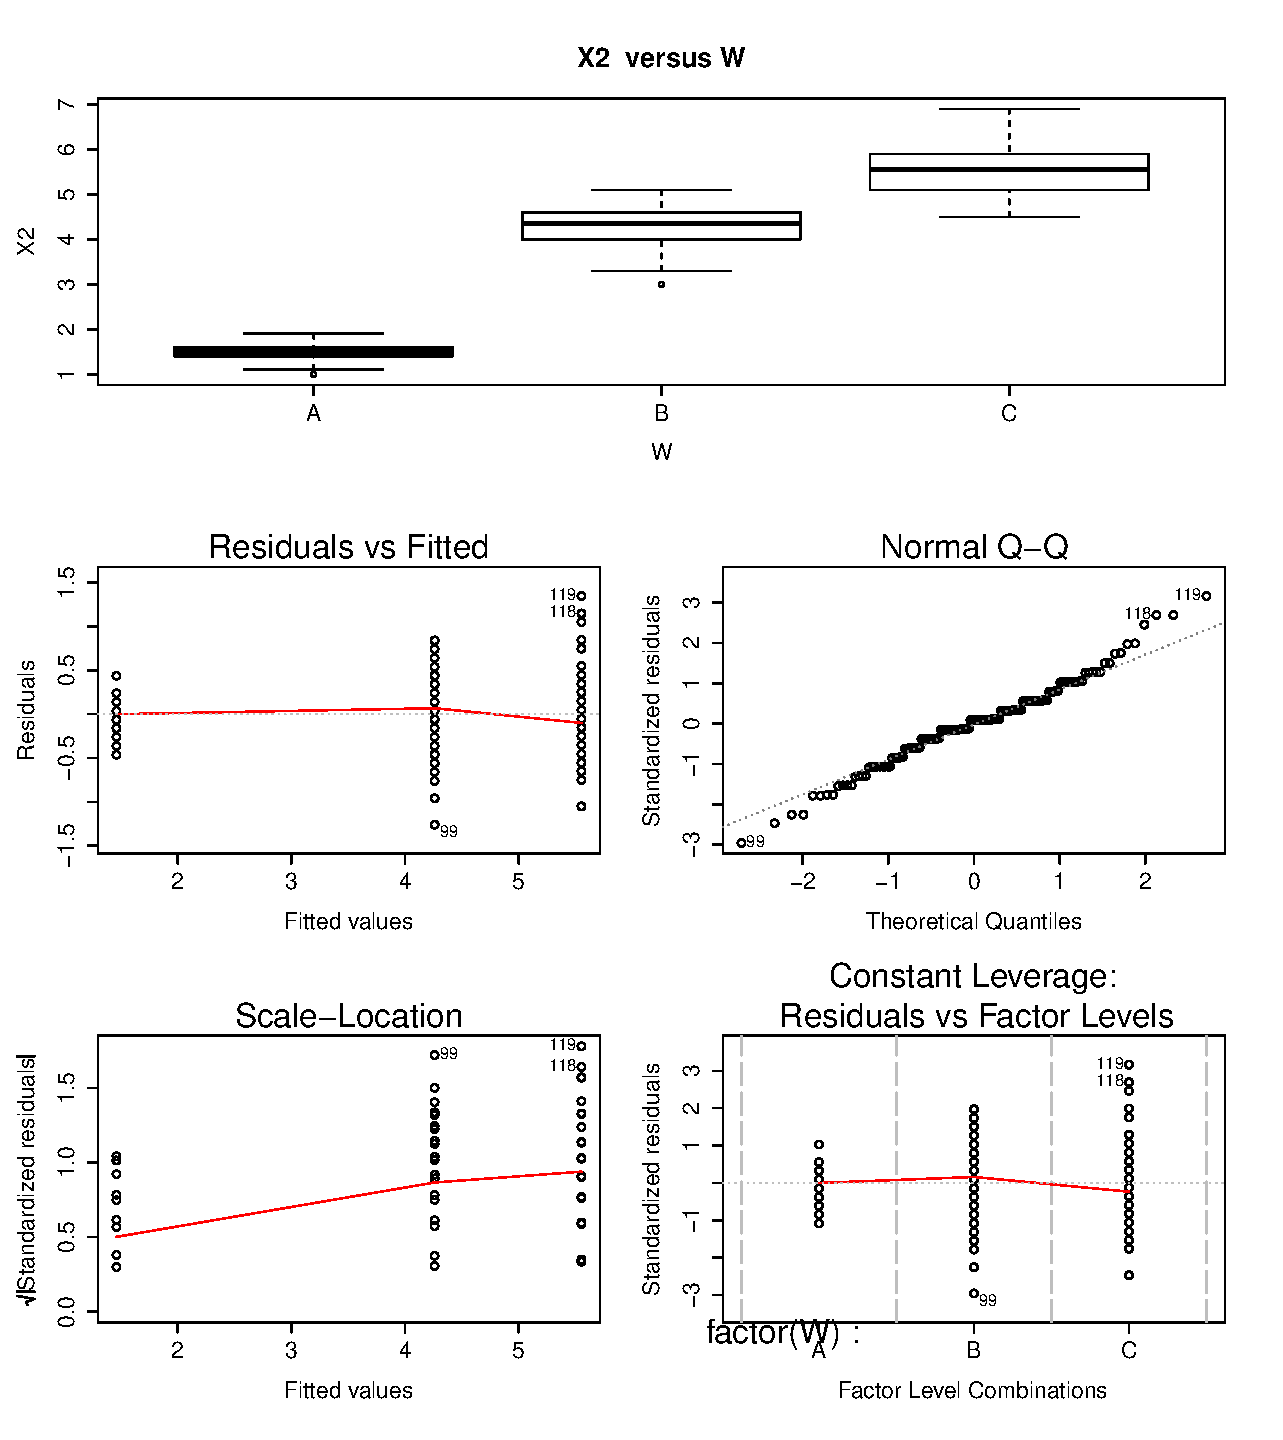
\includegraphics[scale=0.6]{X2vsW.eps}
  \caption{W vs X2}
  \label{fig:X2vsW}
  \end{figure}
  
  \item W vs X3
  \begin{lstlisting}
"Fitted model:"
Call:
   aov(formula = data[[col]] ~ factor(W), data = data)

Terms:
                factor(W) Residuals
Sum of Squares   80.41333   6.15660
Deg. of Freedom         2       147

Residual standard error: 0.20465
Estimated effects may be unbalanced
  \end{lstlisting}
  
  \begin{lstlisting}
"Anova table:"
             Df Sum Sq Mean Sq F value Pr(>F)    
factor(W)     2  80.41   40.21     960 <2e-16 ***
Residuals   147   6.16    0.04                   
---
Signif. codes:  0 ‘***’ 0.001 ‘**’ 0.01 ‘*’ 0.05 ‘.’ 0.1 ‘ ’ 1
  \end{lstlisting}
  
  According to the ANOVA table above, the X3 variable does not have the same
  mean for all values of W. This is also clear on the plot in
  figure~\ref{fig:X3vsW} (p.~\pageref{fig:X3vsW}).
  
  \begin{figure}[H]
  \centering
  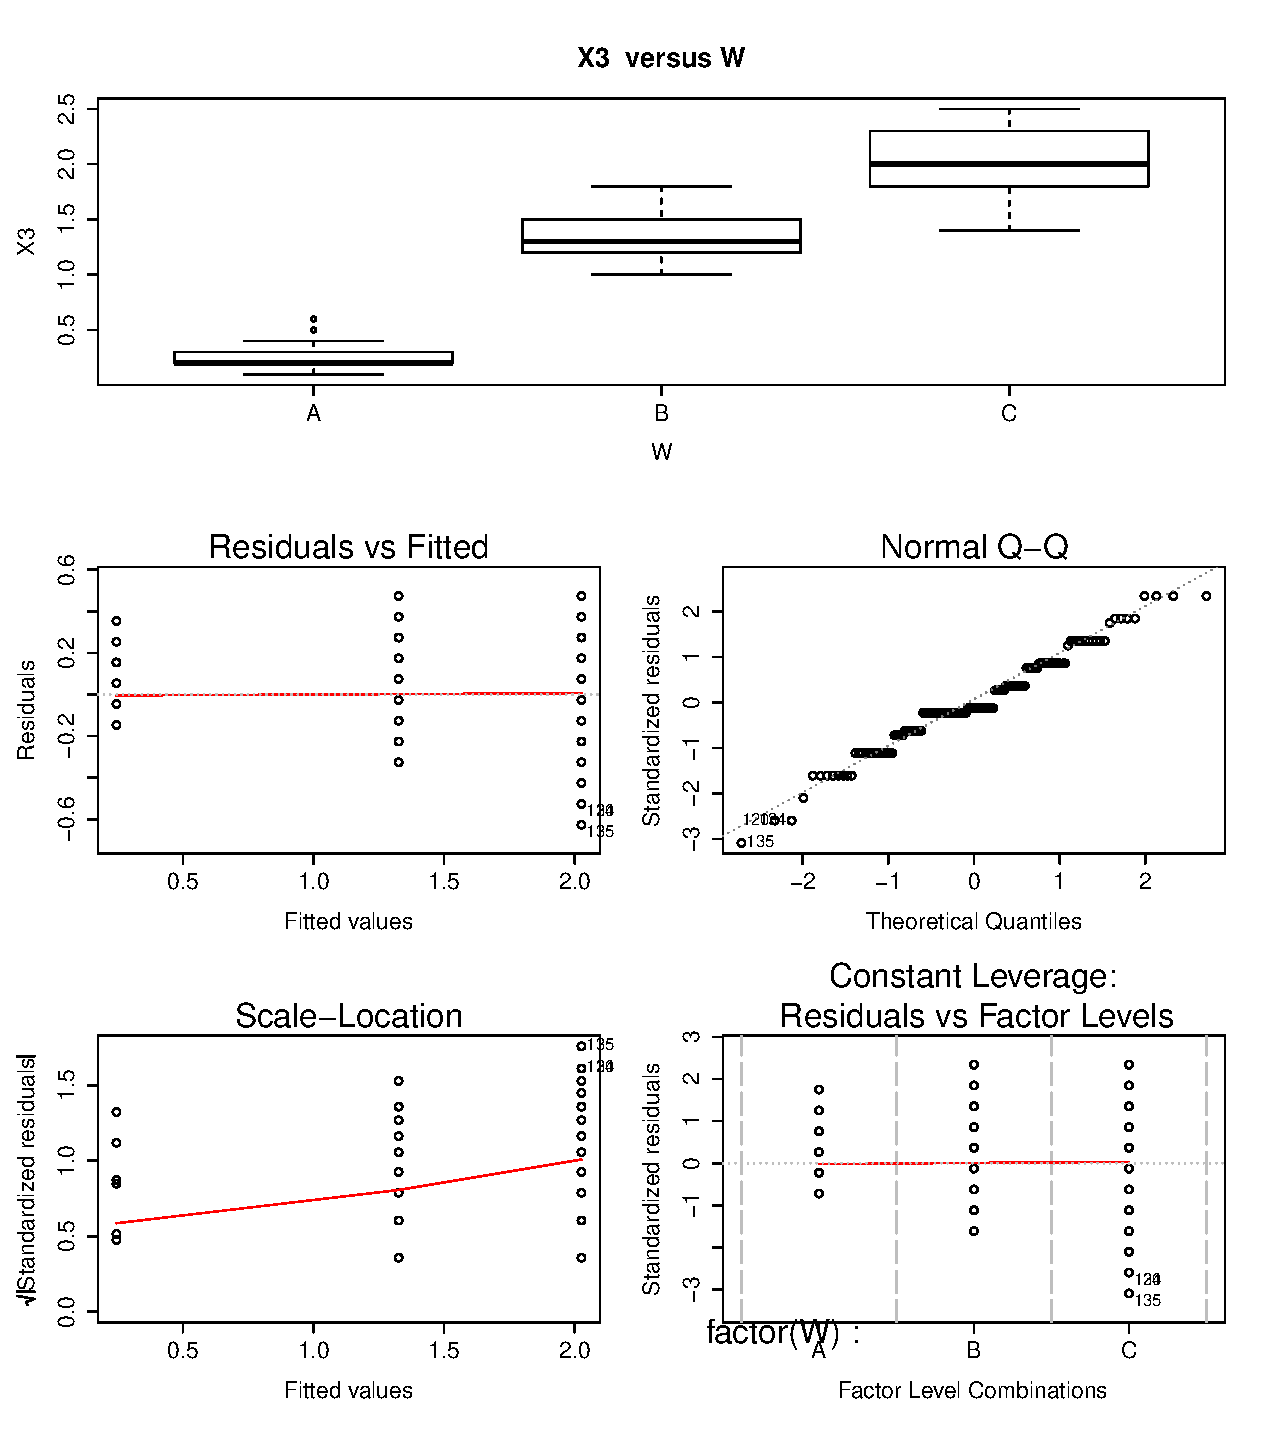
\includegraphics[scale=0.6]{X3vsW.eps}
  \caption{W vs X3}
  \label{fig:X3vsW}
  \end{figure}
\end{enumerate}

\subsubsection{}
Check the assumptions and provide alternatives when the assumptions are violated

\begin{enumerate}
  \item W vs Y
  We will use the Shapiro-Wilk test to check the normality of the residuals:
  \begin{lstlisting}
"Shapiro-Wilk test for normality of residuals:"

	Shapiro-Wilk normality test

data:  fit$residuals
W = 0.9879, p-value = 0.2189
  \end{lstlisting}
  
  The test confirms what we see on the NPP plot in figure~\ref{fig:YvsW}; the
  residuals are from a normal distribution.
  
  Next we will check the homogenity of the variance among the diffrerent values
  of W with the Bartlett test:
  \begin{lstlisting}
"Homogenity of variances:"

	Bartlett test of homogeneity of variances

data:  data[[col]] by factor(W)
Bartlett's K-squared = 16.006, df = 2, p-value = 0.0003345
  \end{lstlisting}
  
  The test reports that the variance is not the same and we can also observe
  that on the box and leverage plot in figure~\ref{fig:YvsW}.
  
  \item W vs X1
  We will use the Shapiro-Wilk test to check the normality of the residuals:
  \begin{lstlisting}
"Shapiro-Wilk test for normality of residuals:"

	Shapiro-Wilk normality test

data:  fit$residuals
W = 0.98948, p-value = 0.323
  \end{lstlisting}
  The test confirms what we see on the NPP plot in figure~\ref{fig:X1vsW}; the
  residuals are from a normal distribution.
  
  Next we will check the homogenity of the variance among the diffrerent values
  of W with the Bartlett test:
  \begin{lstlisting}
"Homogenity of variances:"

	Bartlett test of homogeneity of variances

data:  data[[col]] by factor(W)
Bartlett's K-squared = 2.0911, df = 2, p-value = 0.3515
  \end{lstlisting}
  The test reports that the variance is the same thus the assumptions for the
  analysis of variance are correct.
  
  \item W vs X2
  We will use the Shapiro-Wilk test to check the normality of the residuals:
  \begin{lstlisting}
"Shapiro-Wilk test for normality of residuals:"

	Shapiro-Wilk normality test

data:  fit$residuals
W = 0.98108, p-value = 0.03676
  \end{lstlisting}
  The test indicates that the residuals are not normally distributed.
  
  Next we will check the homogenity of the variance among the diffrerent values
  of W with the Bartlett test:
  \begin{lstlisting}
"Homogenity of variances:"

	Bartlett test of homogeneity of variances

data:  data[[col]] by factor(W)
Bartlett's K-squared = 5
  \end{lstlisting}
  The test reports that the variance is not the same and we can also observe
  that on the box and leverage plot in figure~\ref{fig:X2vsW}.
  
  \item W vs X3
  We will use the Shapiro-Wilk test to check the normality of the residuals:
  \begin{lstlisting}
"Shapiro-Wilk test for normality of residuals:"

	Shapiro-Wilk normality test

data:  fit$residuals
W = 0.97217, p-value = 0.003866
  \end{lstlisting}
  The test indicates that the residuals are not normally distributed.
  
  Next we will check the homogenity of the variance among the diffrerent values
  of W with the Bartlett test:  
  \begin{lstlisting}
"Homogenity of variances:"

	Bartlett test of homogeneity of variances

data:  data[[col]] by factor(W)
Bartlett's K-squared = 39.213, df = 2, p-value = 3.055e-09
  \end{lstlisting}
  The test reports that the variance is not the same and we can also observe
  that on the box and leverage plot in figure~\ref{fig:X3vsW}.
\end{enumerate}

\subsubsection{}
If significant mean diferences exist, then use two different ad-hoc methods to
identify the mean grouping versus the levels of the categorical variable

\begin{enumerate}
  \item W vs Y
  The mean differences are significant in this case. We will use the Tukey
  honestly significant differences method and the pairwiase t-test to identify
  the difference in means:
  \begin{lstlisting}
Tukey multiple comparisons of means
    95% family-wise confidence level

Fit: aov(formula = data[[col]] ~ factor(W), data = data)

$`factor(W)`
     diff       lwr       upr p adj
B-A 0.930 0.6862273 1.1737727     0
C-A 1.582 1.3382273 1.8257727     0
C-B 0.652 0.4082273 0.8957727     0
  \end{lstlisting}
  
  \begin{lstlisting}
	Pairwise comparisons using t tests with pooled SD 

data:  data[["Y"]] and data[["W"]] 

  A       B      
B 1.8e-15 -      
C < 2e-16 2.8e-09

P value adjustment method: holm 
  \end{lstlisting}
  
  \item W vs X1
  The mean differences are significant in this case. We will use the Tukey
  honestly significant differences method and the pairwiase t-test to identify
  the difference in means:
  \begin{lstlisting}
  Tukey multiple comparisons of means
    95% family-wise confidence level

Fit: aov(formula = data[[col]] ~ factor(W), data = data)

$`factor(W)`
      diff         lwr        upr     p adj
B-A -0.658 -0.81885528 -0.4971447 0.0000000
C-A -0.454 -0.61485528 -0.2931447 0.0000000
C-B  0.204  0.04314472  0.3648553 0.0087802
  \end{lstlisting}
  
  \begin{lstlisting}
	Pairwise comparisons using t tests with pooled SD 

data:  data[["X1"]] and data[["W"]] 

  A       B     
B < 2e-16 -     
C 9.1e-10 0.0031

P value adjustment method: holm
  \end{lstlisting}
  
  \item W vs X2
  The mean differences are significant in this case. We will use the Tukey
  honestly significant differences method and the pairwiase t-test to identify
  the difference in means:
  \begin{lstlisting}
  Tukey multiple comparisons of means
    95% family-wise confidence level

Fit: aov(formula = data[[col]] ~ factor(W), data = data)

$`factor(W)`
     diff     lwr     upr p adj
B-A 2.798 2.59422 3.00178     0
C-A 4.090 3.88622 4.29378     0
C-B 1.292 1.08822 1.49578     0
  \end{lstlisting}
  
  \begin{lstlisting}
	Pairwise comparisons using t tests with pooled SD 

data:  data[["X2"]] and data[["W"]] 

  A      B     
B <2e-16 -     
C <2e-16 <2e-16

P value adjustment method: holm 
  \end{lstlisting}
  
  \item W vs X3
  The mean differences are significant in this case. We will use the Tukey
  honestly significant differences method and the pairwiase t-test to identify
  the difference in means:
  \begin{lstlisting}
  Tukey multiple comparisons of means
    95% family-wise confidence level

Fit: aov(formula = data[[col]] ~ factor(W), data = data)

$`factor(W)`
    diff       lwr       upr p adj
B-A 1.08 0.9830903 1.1769097     0
C-A 1.78 1.6830903 1.8769097     0
C-B 0.70 0.6030903 0.7969097     0
  \end{lstlisting}
  
  \begin{lstlisting}
	Pairwise comparisons using t tests with pooled SD 

data:  data[["X3"]] and data[["W"]] 

  A      B     
B <2e-16 -     
C <2e-16 <2e-16

P value adjustment method: holm
  \end{lstlisting}
\end{enumerate}

\subsection{}
Run the non-parametric one-way ANOVA of each of the continuous variables ($Y,
X_1, X_2, X_3$) on the categorical variable ($W$)

The Kruskal-Wallis is the non-parametric one-way ANOVA test.
\begin{enumerate}
  \item W vs Y
  \begin{lstlisting}
  	Kruskal-Wallis rank sum test

data:  data[["Y"]] by data[["W"]]
Kruskal-Wallis chi-squared = 96.937, df = 2, p-value < 2.2e-16
  \end{lstlisting}
  \item W vs X1
  \begin{lstlisting}
	Kruskal-Wallis rank sum test

data:  data[["X1"]] by data[["W"]]
Kruskal-Wallis chi-squared = 63.571, df = 2, p-value = 1.569e-14
  \end{lstlisting}
  \item W vs X2
  \begin{lstlisting}
	Kruskal-Wallis rank sum test

data:  data[["X2"]] by data[["W"]]
Kruskal-Wallis chi-squared = 130.41, df = 2, p-value < 2.2e-16
  \end{lstlisting}
  \item W vs X3
  \begin{lstlisting}
	Kruskal-Wallis rank sum test

data:  data[["X3"]] by data[["W"]]
Kruskal-Wallis chi-squared = 131.19, df = 2, p-value < 2.2e-16
  \end{lstlisting}
\end{enumerate}

\subsection{}
Provide a scatter-plot matrix of $Y, X_1, X_2, X_3$
  \begin{figure}[H]
  \centering
  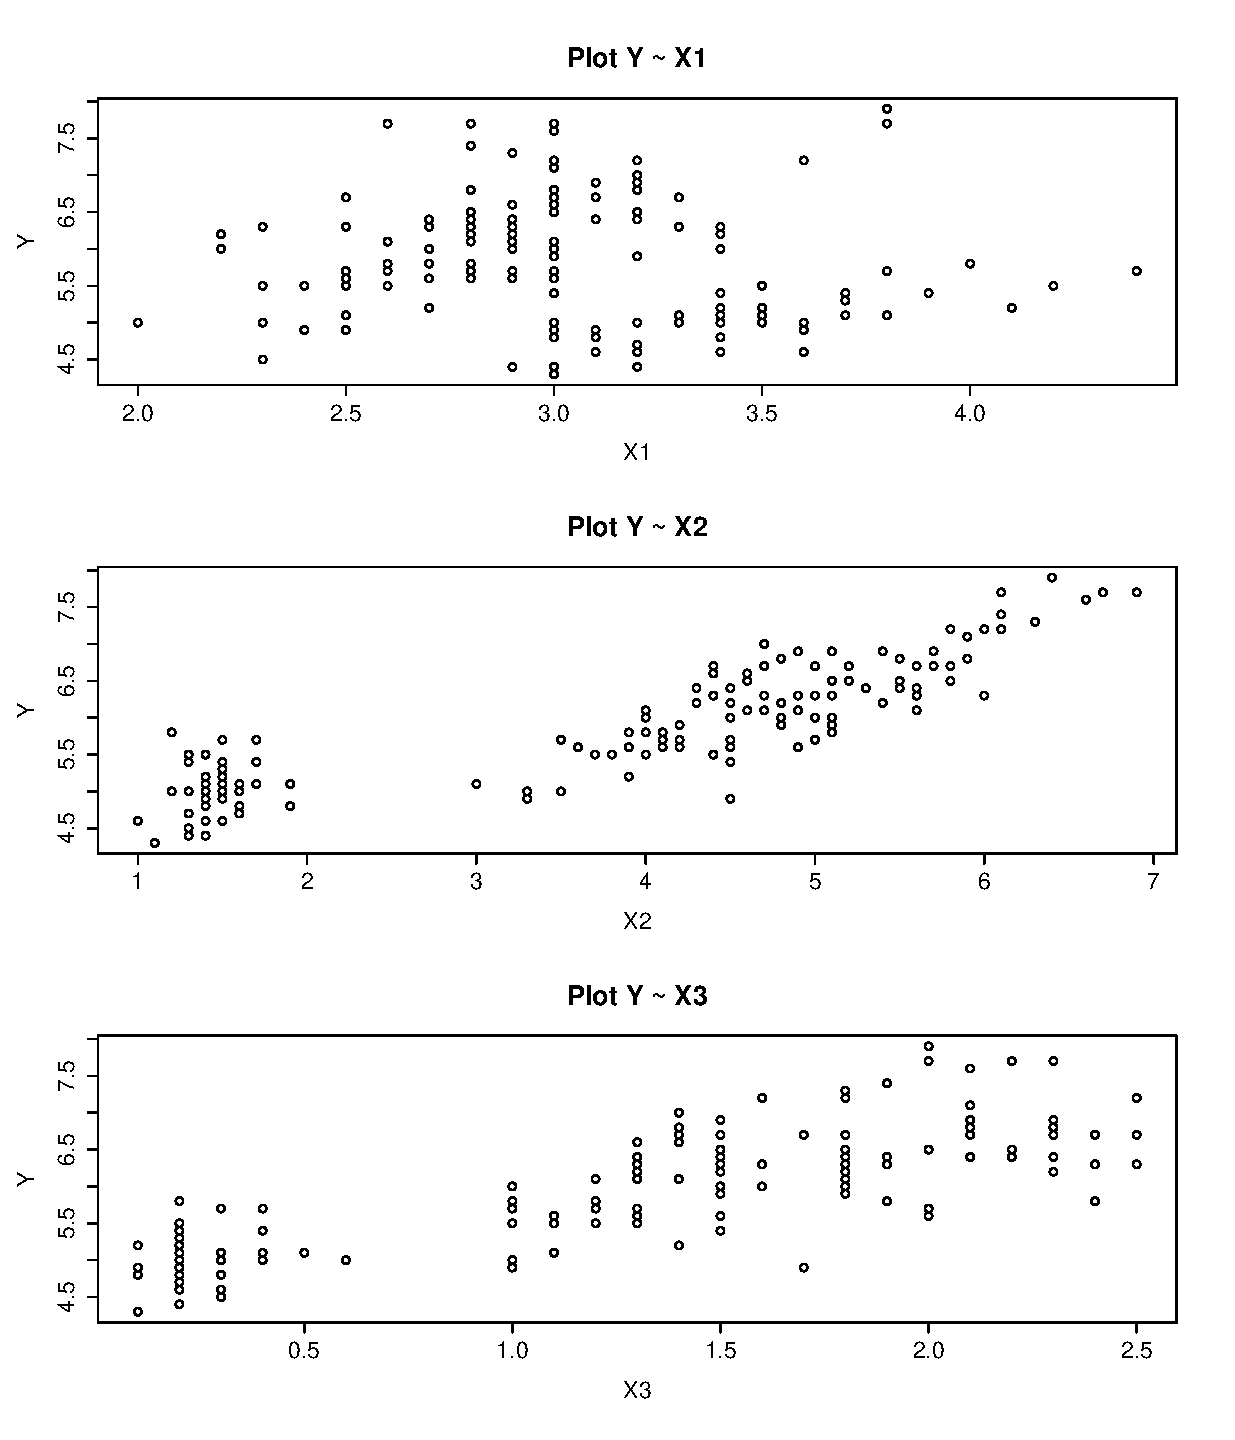
\includegraphics[scale=0.6]{scatter.eps}
  \caption{Scatter plot of continuous variables}
  \label{fig:scatter}
  \end{figure}

\subsection{}
Provide a scatter-plot matrix of $Y, X_1, X_2, X_3$, annotating the different
levels of W in each plot using a different color.

  \begin{figure}[H]
  \centering
  \includegraphics[scale=0.6]{scattercolors.eps}
  \caption{Scatter plot of continuous variables with coloured levels of W}
  \label{fig:scattercolors}
  \end{figure}

\subsection{}
Run the regression model of $Y$ on all the remaining variables ($X_1, X_2, X_3,
W$), including the non-additive terms (i.e. interactions of the continuous
predictors with the categorical)

  \begin{lstlisting}
Call:
lm(formula = Y ~ X1 + X2 + X3 + W + X1:W + X2:W + X3:W, data = data)

Residuals:
     Min       1Q   Median       3Q      Max 
-0.73883 -0.21607  0.00051  0.21813  0.74427 

Coefficients:
            Estimate Std. Error t value Pr(>|t|)    
(Intercept)   2.3519     0.4965   4.737 5.33e-06 ***
X1            0.6548     0.1168   5.605 1.09e-07 ***
X2            0.2376     0.2629   0.904   0.3678    
X3            0.2521     0.4384   0.575   0.5661    
WB           -0.4564     0.6727  -0.678   0.4987    
WC           -1.6520     0.7067  -2.338   0.0208 *  
X1:WB        -0.2680     0.2172  -1.234   0.2194    
X1:WC        -0.3245     0.2016  -1.610   0.1098    
X2:WB         0.6708     0.3017   2.223   0.0278 *  
X2:WC         0.7080     0.2765   2.561   0.0115 *  
X3:WB        -0.9313     0.5866  -1.588   0.1146    
X3:WC        -0.4219     0.4765  -0.885   0.3775    
---
Signif. codes:  0 ‘***’ 0.001 ‘**’ 0.01 ‘*’ 0.05 ‘.’ 0.1 ‘ ’ 1

Residual standard error: 0.2997 on 138 degrees of freedom
Multiple R-squared:  0.8787,	Adjusted R-squared:  0.869 
F-statistic: 90.87 on 11 and 138 DF,  p-value: < 2.2e-16
  \end{lstlisting}
  
\subsection{}
Examine the regression assumptions and provide alternatives if any of them
fails. Also provide a discussion of potential outliers and in uential points (if
any).

  \begin{figure}[H]
  \centering
  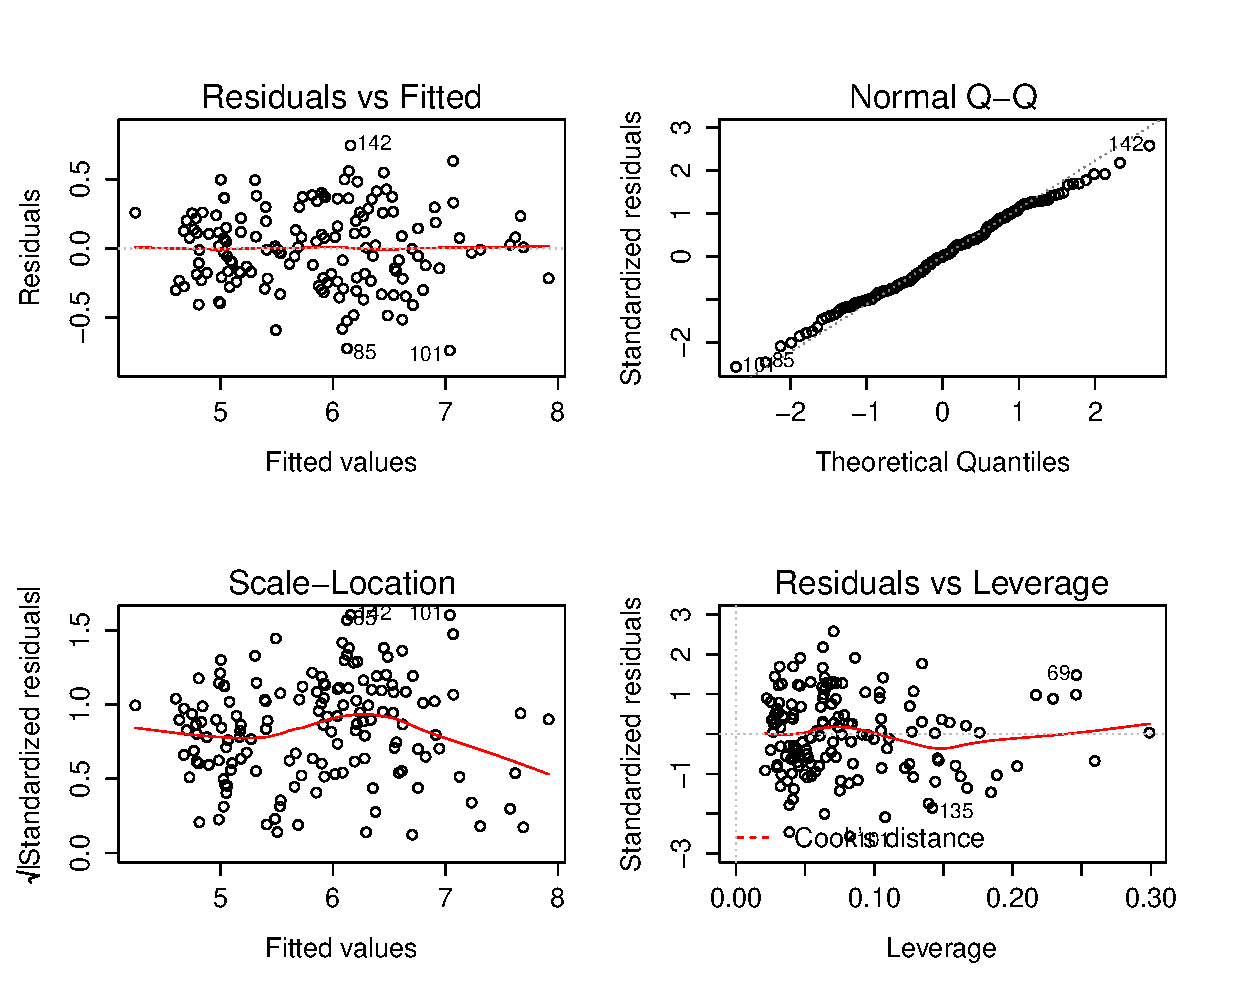
\includegraphics[scale=0.6]{fittedmodel1.eps}
  \caption{Fitted Model}
  \label{fig:fittedmodel1}
  \end{figure}

We can see on the plot in figure~\ref{fig:fittedmodel1} that the residuals are
independent of the predictor variables. They are a ``cloud'' with mean close to
0.

  \begin{lstlisting}
	Shapiro-Wilk normality test

data:  fit$residuals
W = 0.99341, p-value = 0.7269
  \end{lstlisting}
  
From the Q-Q plot and the Shapiro-Wilk test above we can confirm that the
residuals are normally distributed.

\subsection{}
Use the ``stepwise regression'' and the ``all subset'' approach to examine
whether you can reduce the dimension of the model.

\begin{enumerate}
  \item Stepwise regression
  \begin{lstlisting}
Start:  AIC=-55.6
Y ~ 1

       Df Sum of Sq     RSS      AIC
+ X2    1    77.643  24.525 -267.641
+ X3    1    68.353  33.815 -219.460
+ W     2    63.212  38.956 -196.230
+ X1    1     1.412 100.756  -55.690
<none>              102.168  -55.602

Step:  AIC=-267.64
Y ~ X2

       Df Sum of Sq     RSS     AIC
+ X1    1     8.196  16.329 -326.66
+ W     2     7.843  16.682 -321.45
+ X3    1     0.644  23.881 -269.63
<none>               24.525 -267.64
- X2    1    77.643 102.168  -55.60

Step:  AIC=-326.66
Y ~ X2 + X1

       Df Sum of Sq     RSS     AIC
+ W     2     2.363  13.966 -346.11
+ X3    1     1.883  14.445 -343.04
<none>               16.329 -326.66
- X1    1     8.196  24.525 -267.64
- X2    1    84.427 100.756  -55.69

Step:  AIC=-346.11
Y ~ X2 + X1 + W

       Df Sum of Sq    RSS     AIC
+ X3    1    0.4090 13.556 -348.57
+ X2:W  2    0.5817 13.384 -348.49
+ X1:W  2    0.5641 13.402 -348.29
<none>              13.966 -346.11
- W     2    2.3632 16.329 -326.66
- X1    1    2.7161 16.682 -321.45
- X2    1   14.0382 28.004 -243.74

Step:  AIC=-348.57
Y ~ X2 + X1 + W + X3

       Df Sum of Sq    RSS     AIC
+ X2:W  2    0.4883 13.068 -350.07
+ X1:W  2    0.3848 13.172 -348.88
+ X3:W  2    0.3720 13.184 -348.74
<none>              13.556 -348.57
- X3    1    0.4090 13.966 -346.11
- W     2    0.8889 14.445 -343.04
- X1    1    3.1250 16.681 -319.45
- X2    1   13.7853 27.342 -245.33

Step:  AIC=-350.07
Y ~ X2 + X1 + W + X3 + X2:W

       Df Sum of Sq    RSS     AIC
+ X1:W  2    0.4398 12.628 -351.20
+ X3:W  2    0.3875 12.681 -350.58
<none>              13.068 -350.07
- X2:W  2    0.4883 13.556 -348.57
- X3    1    0.3156 13.384 -348.49
- X1    1    3.2285 16.297 -318.95

Step:  AIC=-351.2
Y ~ X2 + X1 + W + X3 + X2:W + X1:W

       Df Sum of Sq    RSS     AIC
- X3    1   0.14311 12.771 -351.51
<none>              12.628 -351.20
- X1:W  2   0.43978 13.068 -350.07
+ X3:W  2   0.23370 12.395 -350.00
- X2:W  2   0.54329 13.172 -348.88

Step:  AIC=-351.51
Y ~ X2 + X1 + W + X2:W + X1:W

       Df Sum of Sq    RSS     AIC
<none>              12.771 -351.51
+ X3    1   0.14311 12.628 -351.20
- X1:W  2   0.61227 13.384 -348.49
- X2:W  2   0.62995 13.402 -348.29

Call:
lm(formula = Y ~ X2 + X1 + W + X2:W + X1:W, data = data)

Coefficients:
(Intercept)           X2           X1           WB           WC        X2:WB        X2:WC        X1:WB        X1:WC  
     2.3037       0.2834       0.6674      -0.1873      -1.6790       0.4522       0.6514      -0.4198      -0.4075  
  \end{lstlisting}
  The formula that we get with Stepwise regression is $Y ~ X_1 + X_2 + W +
  X_1:W + X_2:W$
  
  \item All subset
  \begin{lstlisting}
Subset selection object
Call: regsubsets.formula(Y ~ X1 + X2 + X3 + W + X1:W + X2:W + X3:W, 
    data = data, nbest = 1)
11 Variables  (and intercept)
      Forced in Forced out
X1        FALSE      FALSE
X2        FALSE      FALSE
X3        FALSE      FALSE
WB        FALSE      FALSE
WC        FALSE      FALSE
X1:WB     FALSE      FALSE
X1:WC     FALSE      FALSE
X2:WB     FALSE      FALSE
X2:WC     FALSE      FALSE
X3:WB     FALSE      FALSE
X3:WC     FALSE      FALSE
1 subsets of each size up to 8
Selection Algorithm: exhaustive
         X1  X2  X3  WB  WC  X1:WB X1:WC X2:WB X2:WC X3:WB X3:WC
1  ( 1 ) " " "*" " " " " " " " "   " "   " "   " "   " "   " "  
2  ( 1 ) "*" "*" " " " " " " " "   " "   " "   " "   " "   " "  
3  ( 1 ) "*" "*" "*" " " " " " "   " "   " "   " "   " "   " "  
4  ( 1 ) "*" "*" " " " " "*" " "   " "   " "   " "   "*"   " "  
5  ( 1 ) "*" "*" " " " " "*" " "   "*"   " "   " "   "*"   " "  
6  ( 1 ) "*" " " " " " " "*" "*"   "*"   "*"   "*"   " "   " "  
7  ( 1 ) "*" " " " " " " "*" "*"   "*"   "*"   "*"   "*"   " "  
8  ( 1 ) "*" "*" " " " " "*" "*"   "*"   "*"   "*"   "*"   " "  
  \end{lstlisting}
  \begin{figure}[H]
  \centering
  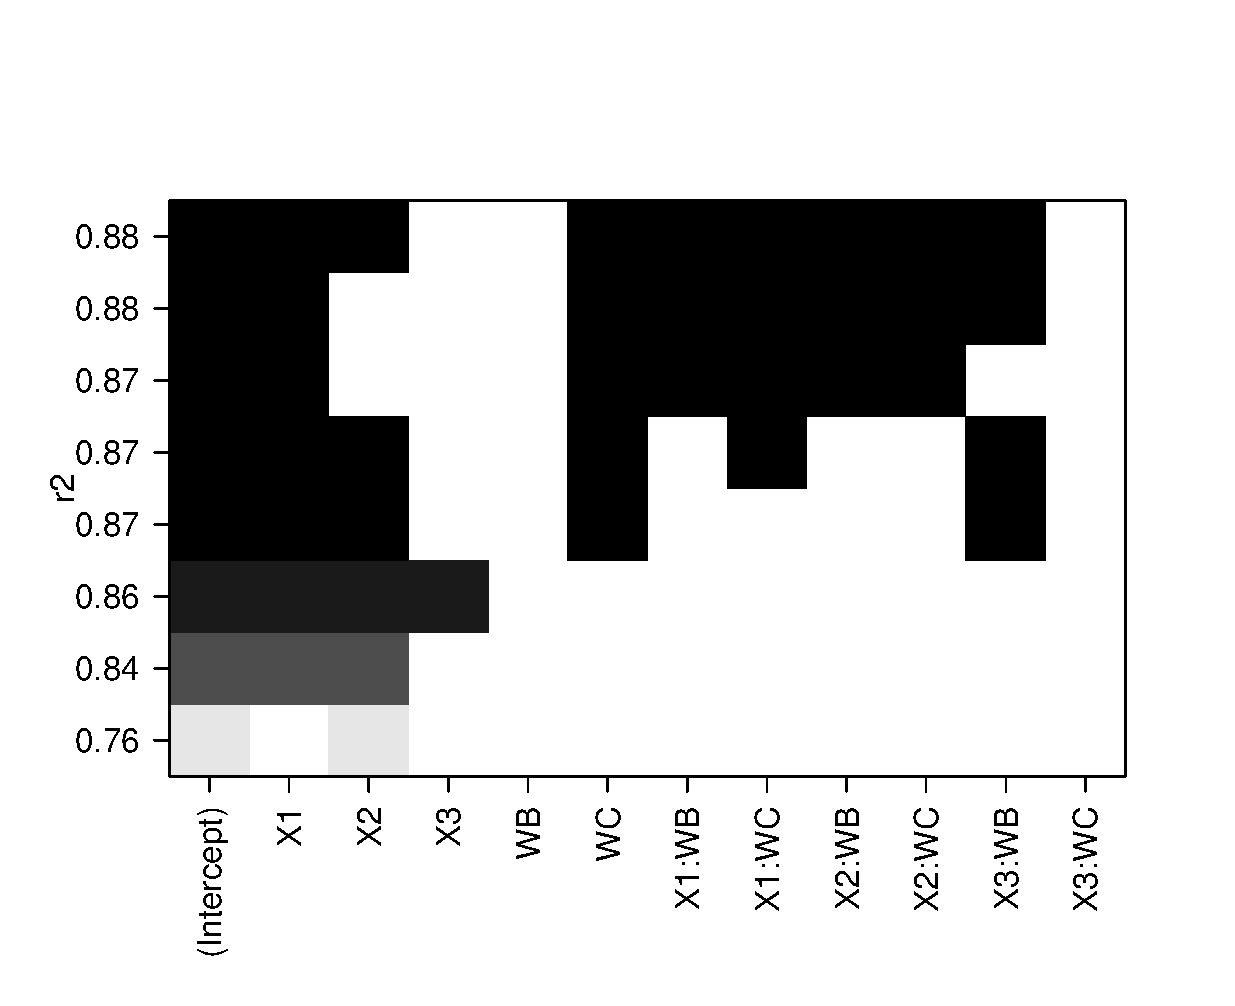
\includegraphics[scale=0.6]{allsubsets.eps}
  \caption{All Subsets result}
  \label{fig:allsubsets}
  \end{figure}
\end{enumerate}

\subsection{}
Use the ANOVA F-test to examine which is the ``best'' sub-model.

For the model $Y ~ X_1 + X_2 + W + X_1:W + X_2:W$ the anova test yields:
  \begin{lstlisting}
Analysis of Variance Table

Response: Y
           Df Sum Sq Mean Sq  F value    Pr(>F)    
X2          1 77.643  77.643 857.1976 < 2.2e-16 ***
X1          1  8.196   8.196  90.4885 < 2.2e-16 ***
W           2  2.363   1.182  13.0454 6.336e-06 ***
X2:W        2  0.582   0.291   3.2113   0.04327 *  
X1:W        2  0.612   0.306   3.3798   0.03684 *  
Residuals 141 12.772   0.091                       
---
Signif. codes:  0 ‘***’ 0.001 ‘**’ 0.01 ‘*’ 0.05 ‘.’ 0.1 ‘ ’ 1
  \end{lstlisting}

\subsection{}
Using the model found in the previous subsection provide a point estimate and a
$95\%$ confidence interval for the prediction of $Y$ when: $(X_1, X_2, X_3,
W)=(3.1,3.75,1.2,A)$

The predicted value is $Y = 5.435551$


\end{document}
